\documentclass[11pt]{standalone}
\usepackage{tikz}
\usepackage{amssymb}
\begin{document}
% GEOMIRA export: TikZ. One unit is 60bp (80 px on screen).
% Needs \usepackage{tikz} and \usepackage{amssymb}.
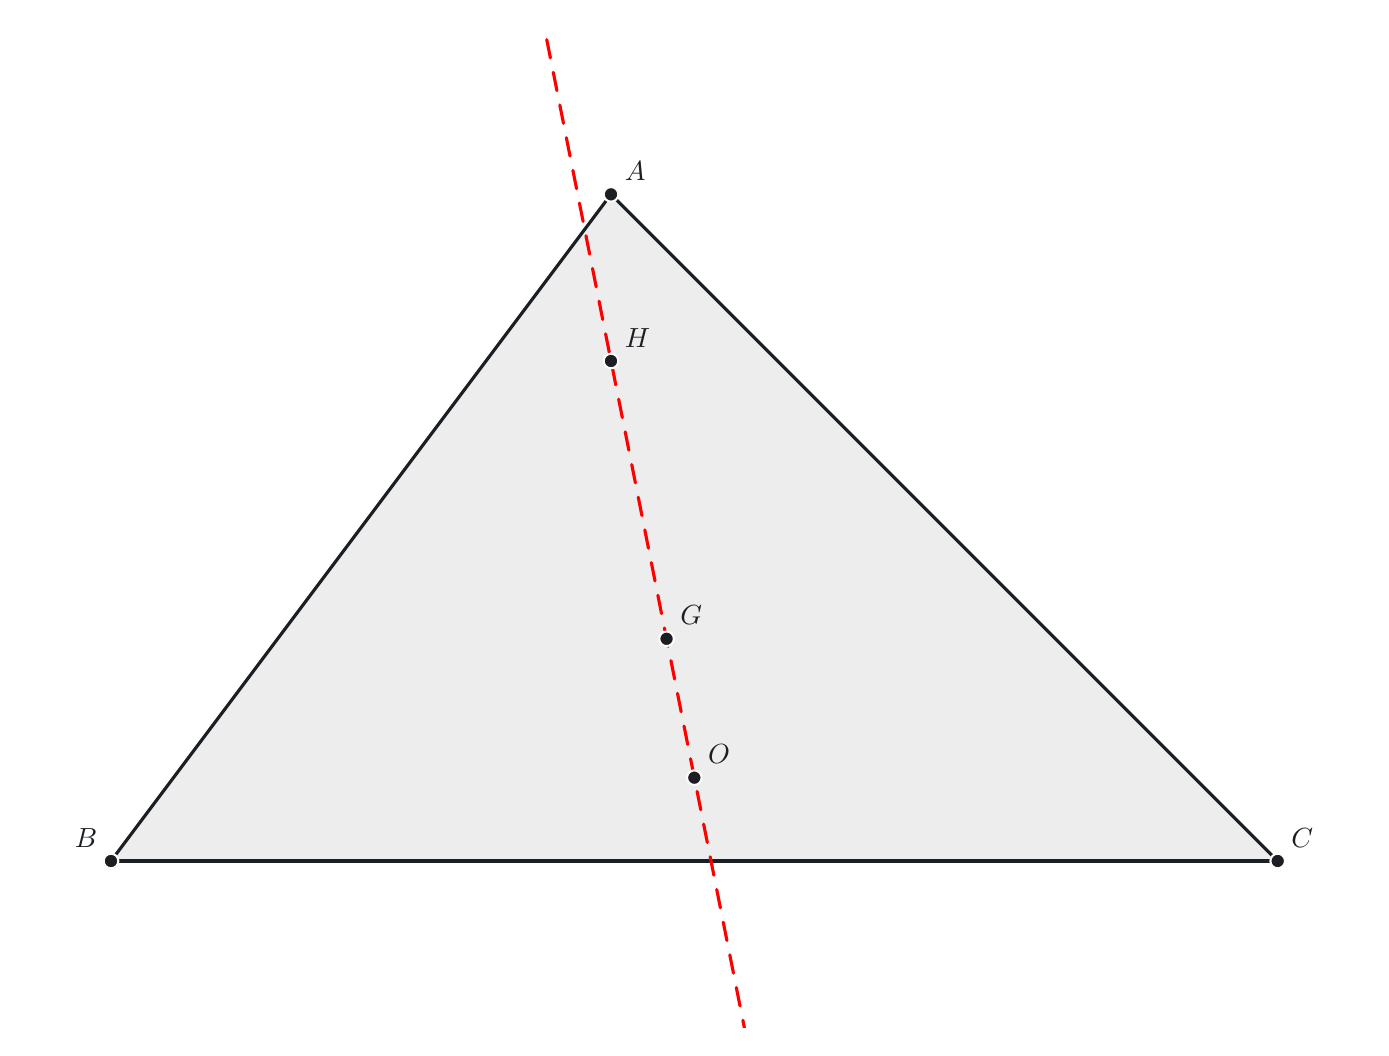
\begin{tikzpicture}[x=60bp, y=60bp, line cap=round, line join=round]
\definecolor{gmc0}{HTML}{1B1F24}
\definecolor{gmc1}{HTML}{FF0000}
\definecolor{gmc2}{HTML}{FBFBF8}
\clip (-2.5,-1) rectangle (5.5,5);
% abc
\fill[gmc0, fill opacity=0.08] (1,4) -- (-2,0) -- (5,0) -- cycle;
\draw[gmc0, line width=1.125bp] (1,4) -- (-2,0);
\draw[gmc0, line width=1.125bp] (-2,0) -- (5,0);
\draw[gmc0, line width=1.125bp] (5,0) -- (1,4);
% e
\draw[gmc1, line width=1.125bp, dash pattern=on 6.75bp off 5.25bp] (1.97,-1.85) -- (0.43,5.85);
% A
\filldraw[fill=gmc0, draw=gmc2, line width=0.75bp] (1,4) circle[radius=2.625bp];
% B
\filldraw[fill=gmc0, draw=gmc2, line width=0.75bp] (-2,0) circle[radius=2.625bp];
% C
\filldraw[fill=gmc0, draw=gmc2, line width=0.75bp] (5,0) circle[radius=2.625bp];
% O
\filldraw[fill=gmc0, draw=gmc2, line width=0.75bp] (1.5,0.5) circle[radius=2.625bp];
% G
\filldraw[fill=gmc0, draw=gmc2, line width=0.75bp] (1.3333,1.3333) circle[radius=2.625bp];
% H
\filldraw[fill=gmc0, draw=gmc2, line width=0.75bp] (1,3) circle[radius=2.625bp];
\node[anchor=south west, inner sep=0pt, text=gmc0] at (1.0795,4.0795) {$A$}; % label of A
\node[anchor=south east, inner sep=0pt, text=gmc0] at (-2.0795,0.0795) {$B$}; % label of B
\node[anchor=south west, inner sep=0pt, text=gmc0] at (5.0795,0.0795) {$C$}; % label of C
\node[anchor=south west, inner sep=0pt, text=gmc0] at (1.5795,0.5795) {$O$}; % label of O
\node[anchor=south west, inner sep=0pt, text=gmc0] at (1.4129,1.4129) {$G$}; % label of G
\node[anchor=south west, inner sep=0pt, text=gmc0] at (1.0795,3.0795) {$H$}; % label of H
\end{tikzpicture}
\end{document}
